\section{extended problem}
We shall discuss several problems simular to the foolproof problem in section 1. These are called inference problems. For convenience, we assume fake coins are minor in the whole coins.(e.g. ($\pa\leq \pb $)
In the same way in Section 2, we present a scheme as a graph. There are four inference problems: infering a fake coin,a real coin, real-fake pair, a fake coin and a real coin. We $-$, $+$, $\pm$, $+-$ superscription to denote them seperately.

\subsection*{Infering a real-fake pair}
{
\setlength{\leftskip}{1cm}
\setlength{\rightskip}{1cm}
There are $\pa$ fake coins and $\pb$ real coins ($\pa, \pb > 0$). The real coins are all the same weight and also the counterfeit coins, but two  types are different weight. Each time we compare only two coins have the same weight or not. In this case, assume $\pa$, $\pb$ are known.
Find the smallest number of comparison that we can infer a pair is real-fake. In this problem, we don't need to know which one is fake.\\

}
\begin{definition}
If a scheme could infer a real-fake coin. We say this graph is a inferable$^\pm$ scheme for fake ($\IS^\pm$). Otherwise it's not inferable$^\pm$.

Optimal inferable scheme for fake ($\OIS^\pm$) is $\IS^\pm$ with minimum number of comparison.
Deonte the number of edges of $\OIS^\pm$ by $\tau^\pm(\pa,\pb)$.
\end{definition}

Note that in the foolproof problem. We can infer the pair on the scale which is unbalanced. But sometimes before the unbalance appears, we can infer a pair is real-fake. The following shows the answer is $\tau(\pa,\pb)-1$.

\begin{lemma}
$\OIS^\pm= \text{removing an arbitrary edge}$. That is, $\tau^\pm(a,b)=\tau(a,b)-1$
\end{lemma}

\begin{proof}
We divide the proof of the equation into two inequations. For conciseness, we denote $\tau(a,b)-1$ by $\tau$ and the answer of this problem as $\tau^\pm$.

For a optimal foolproof scheme $G$(with $\tau$ edges). Let $G'$ = ($G$ remove an arbitrary edge $e$), then through $F'$.
If $G'$ has unbalance comparison, we conclude the one is unbalanced, otherwise we could conclude $e$ is unbalanced.
Either case shows $G'$ is sufficient to infer a real-fake pair.
\[\tau^\pm \leq \tau-1\]

If we could infer a pair $e$ is real-fake through the optimal scheme $F$(with $\tau^\pm$ comparisons).
Then the graph $F$ + $e$ is foolproof.
\[\tau\leq \tau^\pm+1\]

From the above inequations, the lemma holds.

\end{proof}
\subsection*{Two conditions of a testing scheme}

When testing a testing scheme, there are two conditions.

\textbf{Condition 1.} there is an unbalanced edges

\textbf{Condition 2.} they are all balanced

For infering a $\pm$, we must ganrantee both conditions work. For Condition 1, we would simplily infer the unbalanced edges. For Condition 2, we would infer the edge must be unbalanced because adding this edge would form a foolproof scheme.
For the following inference problems($-$,$+$,$+-$), we shall use the same logic. 

\subsection*{Infering a fake coin}
{
\setlength{\leftskip}{1cm}
\setlength{\rightskip}{1cm}
\noindent 
There are $\pa$ fake coins and $\pb$ real coins ($\pa, \pb > 0$). The real coins are all the same weight and also the counterfeit coins, but two  types are different weight. Each time we compare only two coins have the same weight or not. In this case, assume $\pa$, $\pb$ are known.
Find the smallest number of comparison that we can infer a coin is fake.\\

}


\begin{definition}
Same as previous problem, we define $\IS^-$, $\OIS^-$ and $\tau^-(a,b)$.
\end{definition}

Note that $\OFS(a,b)$ could find a real and a fake coin. Thus $\tau(\pa,\pb)$ is an upper bound of $\tau^-(\pa,\pb)$.
A $\IS^-(\pa,\pb)$ better than $\OFS(\pa,\pb)$ must use another strategy, which is, though all comparisons result in balance we could still infer a `$-$'.\\

Before solving $\IS^-$, we observe how a inferable$^-$ scheme works.

For a testing scheme, there are two conditions

If \textbf{Condition 1.} happens then we immediate infer the fake coin from the unbalanced.
If \textbf{Condition 2.} happens, we must claim a fake coin, and this coin couldn't be a real one in any condition, otherwise this inference is wrong.\\

We present an optimal inferable$^-$ scheme as a integer partition for an example. Let (a,b)=(2,6), 
this scheme is [3,3,`1',1] .If \textbf{Condition 2}, we infer the `1' is the fake coin. To explain more, we introduce the following lemma.

\begin{lemma}\label{lma:inferable}
If \textbf{Condition 2}, the scheme is inferable for a fake coin $c_1$ if and only if removing $c_1$'s part, the remaining parts avoids $\pa$. Physically, $c_1$ must not be a real coin with \textbf{Condition 2}.
\end{lemma}

To find a inferable$^-$ better than $\OFS$ must solve \textbf{Condition 2}.
Denote the part of the fake coin to be infered as $i(i\leq\pa)$. 
Beyound the remainning $\pa+\pb-i$ parts, 
(1)they must avoid $\pa$, since if there's a subset sum $\pa$, assign the subset `$+$', this claim is wrong
(2)they must contain $\pa-i$ or equivalently contain $\pb$, since there must exist a condition such that the coin is fake and \textbf{Condition 2}.


\begin{definition}
For convenience, we define $Q(n,a,b)$ as the number of edges that avoids $\pa$ but contains $\pb$ 
\end{definition}

Note that $Q(n,a,b)\geq\tau(a,n-a)$\\

For \textbf{Condition 2.}, $1\leq i\leq\pa$ for $\IS^-$, thus we get the following lemma.

\begin{lemma}
$\tau^-(\pa,\pb)=min\{\tau(\pa,\pb), \{i-1+Q(\pa+\pb-i,\pa,\pb) | 1\leq i\leq\pa\} \}$
\end{lemma}

We are ready to solve $\OIS^-$ now.

\begin{theorem}
$\OIS^-(\pa,\pb)=optimal\{\OFS(a,b), \{\text{a tree of i-1 nodes and }\OFS(a,b-i) |1\leq i\leq a\}\}$

$\tau^-(\pa,\pb)=min\{\tau(\pa,\pb), \{i-1+\tau(\pa,\pb-i) | 1\leq i\leq\pa\} \}$
\end{theorem}

\begin{proof}
We divide the proof into inferable$^-$ part and optimal part.

\noindent{\bf (inferable$^-$ Part:)}

For $OFS(a,b)$ could infer a fake coin because only \textbf{Condition 1.} happens.
For $\{\text{a tree of i nodes and }OFS(a,b-i) |1\leq i\leq a\}\}$, if \textbf{Condition 2.}, we infer one coin of the i-node tree as fake coin.

\noindent{\bf (Optimal Part:)}
from lemma 5.2
\begin{align*}
\tau^-(a,b)&=min\{\tau(a,b),\{i-1+Q(a+b-i,a,b) | 1\leq i\leq a\} \}\\
&\geq min\{\tau(a,b), \{i-1+\tau(a,b-i) | 1\leq i\leq a\} \}
\end{align*}

is a optimal lower bound.

And $optimal\{OFS(a,b), \{\text{a tree of i nodes and }OFS(a,b-i) |1\leq i\leq a\}\}$ reaches this lower bound.

\end{proof}

\subsection*{Infering a real coin}

{
\setlength{\leftskip}{1cm}
\setlength{\rightskip}{1cm}
\noindent 
There are $\pa$ fake coins and $\pb$ real coins ($\pa, \pb > 0$). The real coins are all the same weight and also the counterfeit coins, but two  types are different weight. Each time we compare only two coins have the same weight or not. In this case, assume $\pa$, $\pb$ are known.
Find the smallest number of comparison that we can infer a coin is real.\\

}

\begin{definition}
Same as previous problem, we define $\IS^+$, $\OIS^+$ and $\tau^+(a,b)$.
\end{definition}

$\OIS^+$ is trivial.
That is, comparing $\pa$ coins in a group. 

\begin{theorem}
$\OIS^+(\pa,\pb)=\text{a tree of }\pa+1\text{ nodes}$
\end{theorem}
\begin{proof}
We divide the proof into inferable$^+$ part and optimal part.

\noindent{\bf (Inferable$^+$ Part:)}

we omit this part since it's same as previous theorem.

\noindent{\bf (Optimal Part:)}
\begin{align*}
\tau^+(a,b)&=min\{\tau(a,b), \{i-1+Q(a+b-i,b,a) | 1\leq i\leq b\} \}&\\
&\geq min\{\tau(a,b), \{i-1+\tau(a-i,b) | 1\leq i\leq b\} \} &\text{by Theorem 2.2.}\\
&\geq min\{\floor{\frac{a+b}{2}}, i-1+\frac{a-i+b}{2}\}&\\
&\geq min\{a, a\}=a &
\end{align*}

is a optimal lower bound.

$\text{a tree of }\pa+1\text{ nodes}$ reaches optimal lower bound.
\end{proof}

\subsection*{Infering a real coin and a fake coin}

{
\setlength{\leftskip}{1cm}
\setlength{\rightskip}{1cm}
\noindent 
There are $\pa$ fake coins and $\pb$ real coins ($\pa, \pb > 0$). The real coins are all the same weight and also the counterfeit coins, but two  types are different weight. Each time we compare only two coins have the same weight or not. In this case, assume $\pa$, $\pb$ are known.
Find the smallest number of comparison that we can infer a coin is real and another coin is fake.(e.g. a real-fake pair that we know which one is fake)\\

}
\begin{definition}
Same as previous problem, we define $\IS^{+-}$, $\OIS^{+-}$ and $\tau^{+-}(a,b)$.
\end{definition}

This problem seems the same as the foolproof problem, but not exactly. The difference is whether the real-fake pair need to be compared on the scale. For most cases, OFS is optimal for this problem but not all cases. That is, the answer is $\tau$. Consider $(\pa,\pb)=(3,8)$, there's a OFS, [2, 2, 2, 5]. An edge removed, the scheme [2, 2, 2, `4', `1'] is not only inferable$^\pm$ but also $^+-$(`4' and `1').(see explaination in Figure) In this case, the answer is $\tau-1$.
\begin{figure}[!htb]
   \centering
    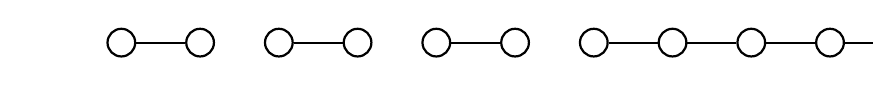
\begin{tikzpicture}[auto, thick]
\tikzstyle{vertex}=[draw,circle,text=violet,minimum width=10pt]
  \foreach \place/\name in {{(0,0)/a},
                            {(1,0)/b},
                            {(2,0)/c},
                            {(3,0)/d},
                            {(4,0)/e},
                            {(5,0)/f},
                            {(6,0)/g},
                            {(7,0)/h},
                            {(8,0)/i},
                            {(9,0)/j},
                            {(10,0)/k}}
    \node[vertex] (\name) at \place {};
  \foreach \source/\dest in {a/b,c/d,e/f,g/h,h/i,i/j,j/k}
      \path (\source) edge (\dest);
\end{tikzpicture} \vspace*{2.5ex}
    \caption{A foolproof scheme for $(\pa,\pb)=(3,8)$}
\end{figure}

\begin{figure}[!htb]
   \centering
    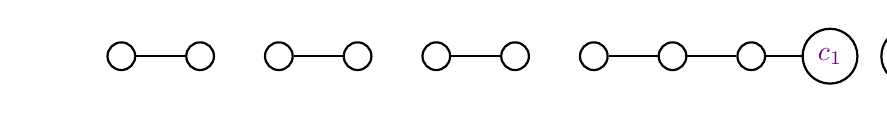
\begin{tikzpicture}[auto, thick]
\tikzstyle{vertex}=[draw,circle,text=violet,minimum width=10pt]
  \foreach \place/\name in {{(0,0)/a},
                            {(1,0)/b},
                            {(2,0)/c},
                            {(3,0)/d},
                            {(4,0)/e},
                            {(5,0)/f},
                            {(6,0)/g},
                            {(7,0)/h},
                            {(8,0)/i}}
    \node[vertex] (\name) at \place {};
  \node[vertex] (j) at (9,0) {$c_1$};
  \node[vertex] (k) at (10,0) {$c_2$};
  \foreach \source/\dest in {a/b,c/d,e/f,g/h,h/i,i/j}
      \path (\source) edge (\dest);
\end{tikzpicture} \vspace*{2.5ex}
    \caption{An $\IS^{+-}$ for $(\pa,\pb)=(3,8)$. If there is an unbalance edge, we infer the fake and real coin of the pair. If edges are all balance, we can infer the coin $c_1$ is real and the coin $c_2$ is fake.}
\end{figure}

Before discussing how to find an $\IS^{+-}$, we observe the range of $\tau^{+-}(a,b)$. Since $\tau(\pa,\pb)$ is sufficient to infer a fake coin and a real coin. 

\[
\tau^{+-} \leq \tau
\]

Through we cound infer a fake coin and a real coin, add this edge into the $\OIS^{+-}$, it's foolproof.

\[
\tau \leq \tau^{+-}+1
\]

Combine the inequations

\[
\tau-1 \leq \tau^{+-} \leq \tau
\]


Before solving $\IS^{+-}$, we observe how this works.

If \textbf{Condition 1.} happens then the solution works.
If \textbf{Condition 2.} happens, we infer a fake coin and a real coin. This pair is not in the $\IS^{+-}$. Adding this pair(edge) into the $\IS^{+-}$, the new graph is foolproof.

\begin{lemma}
Any inferable$^{+-}$ scheme is either a foolproof scheme or a foolproof scheme with an edge removed.
\end{lemma}

\begin{theorem}
Any optimal inferable$^{+-}$ scheme is either a optimal foolproof scheme or an optimal foolproof scheme with an edge removed.
\end{theorem}

Unlike infering a real-fake pair, removing an arbitrary edge from a $\OFS$ may not work.
We enumerate the edge removed for each $\OFS$ then check whether it's inferable$^{+-}$. 
Checking a scheme's inferability$^{+-}$ is similar to checking its inferability$^+$. Condition 1 is simple and the scheme to ganrantee Condition 2 don't happen is $\FS$. We shall focus on Condition 2. If Condition 2 happen can we infer a $+-$? To explain more, we return to the case Figure 4, the reason Figure 4 works is from lemma \ref{lma:inferable}. Because removing $c_1$'s component, the multiset [2,2,2,1] avoids $\pb$